% This file was created with tikzplotlib v0.10.1.
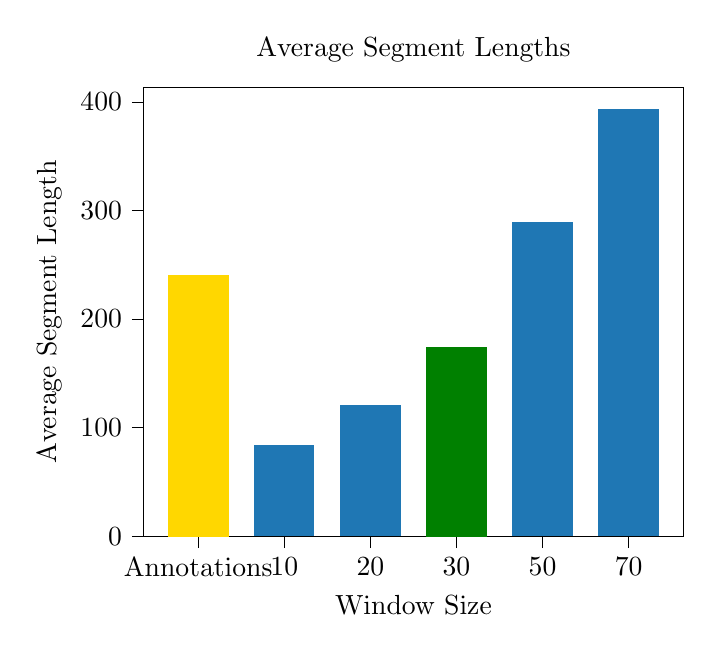
\begin{tikzpicture}

\definecolor{darkgray176}{RGB}{176,176,176}
\definecolor{gold}{RGB}{255,215,0}
\definecolor{green}{RGB}{0,128,0}
\definecolor{steelblue31119180}{RGB}{31,119,180}

\begin{axis}[
tick align=outside,
tick pos=left,
title={Average Segment Lengths},
x grid style={darkgray176},
xlabel={Window Size},
xmin=-6.35, xmax=56.35,
xtick style={color=black},
xtick={0,10,20,30,40,50},
xticklabels={Annotations,10,20,30,50,70},
y grid style={darkgray176},
ylabel={Average Segment Length},
ymin=0, ymax=412.938939685315,
ytick style={color=black}
]
\draw[draw=gold,fill=gold] (axis cs:-3.5,0) rectangle (axis cs:3.5,240.25321888412);
\draw[draw=none,fill=steelblue31119180] (axis cs:6.5,0) rectangle (axis cs:13.5,84.4499744321549);
\draw[draw=none,fill=steelblue31119180] (axis cs:16.5,0) rectangle (axis cs:23.5,121.09860742587);
\draw[draw=green,fill=green] (axis cs:26.5,0) rectangle (axis cs:33.5,173.503223901779);
\draw[draw=none,fill=steelblue31119180] (axis cs:36.5,0) rectangle (axis cs:43.5,289.132817976842);
\draw[draw=none,fill=steelblue31119180] (axis cs:46.5,0) rectangle (axis cs:53.5,393.275180652681);
\end{axis}

\end{tikzpicture}
